\documentclass{article}
\usepackage{amsmath}
\usepackage{amssymb}
\usepackage{graphicx}
\usepackage{hyperref}
\usepackage[version=4]{mhchem}


\begin{document}
In the adjoining figure \(A, B, P\) are tangent points on the circumference of the circle \(O . A M \perp M N, \angle M=\angle N=90^{\circ}\). \(P D\) \(\perp A B\). Show that \(P D^{2}=A M \times B N\).

Solution:
Connect \(A P, B P\).\\
\centering
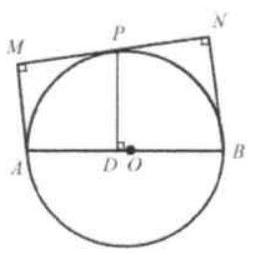
\includegraphics[width=\textwidth]{images/148(5).jpg}

Since \(A B\) is the diameter, \(\angle A P B=90^{\circ}\).\\
Thus \(P D^{2}=A D \times D B\)\\
Since \(\angle M=90^{\circ}\), and \(A M=P M, \angle M A P=\angle M P A=\alpha=\) \(45^{\circ}\).\\
\centering
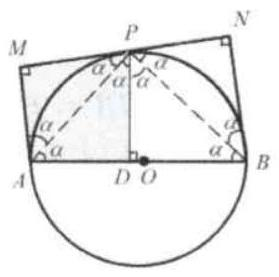
\includegraphics[width=\textwidth]{images/148.jpg}


Since \(\angle N=90^{\circ}\), and \(B N=P N, \angle N P B=\angle N B P=\alpha=45^{\circ}\).\\
So \(\angle B A P=\angle B P N=\alpha=45^{\circ}\) (both angles face the same arc \(P B\) ).\\
Since \(\angle A D P=90^{\circ}, \angle D P A=\angle D A P=\alpha=45^{\circ}\).\\
Similarly \(\angle D P B=\angle D B P=\alpha=45^{\circ}\).

\[
\text { So } \triangle A M P \cong \triangle A D P \quad \Rightarrow \quad A M=A D
\]

So \(\triangle B N P \cong \triangle B D P \quad \Rightarrow \quad B N=D B\) (3)\\
Substituting (2) and (3) into (1): \(P D^{2}=A M \times B N\)\\

\end{document}
